% =====================================================================
% Figure 1 -- PlanGrad-UAV Architecture (matrix-based layout)
%
% Strategy: every sub-module is a cell of a TikZ matrix (5 columns x
% 4 rows). The matrix guarantees alignment; no mixing of absolute and
% relative coordinates. Lane backgrounds are drawn last using fit{}.
%
% Standalone-compilable. Can also be \input from the main document.
% =====================================================================

\definecolor{Cinkblack}{HTML}{1A1A1A}
\definecolor{Crulegrey}{HTML}{B0B5BB}
\definecolor{Cbgblue}{HTML}{E3ECF7}
\definecolor{Cbgyellow}{HTML}{FBF4DC}
\definecolor{Cbggreen}{HTML}{E7F0E5}
\definecolor{Cbggrey}{HTML}{F2F4F7}
\definecolor{Caccorange}{HTML}{E8833A}
\definecolor{Caccnavy}{HTML}{1E3A8A}
\definecolor{Cevtolred}{HTML}{C0524A}
\definecolor{Claneborder}{HTML}{CBD2D9}
\definecolor{Cwindblue}{HTML}{9BB7D4}

\begin{tikzpicture}[
		font=\sffamily\scriptsize,
		>=Stealth,
		every node/.append style={text=Cinkblack},
	]

	% ---------------- Styles ---------------- %
	\tikzset{
		modblock/.style = {
				rectangle, rounded corners=2pt,
				draw=Cinkblack, line width=0.5pt,
				fill=white,
				text width=2.95cm,
				minimum height=1.4cm,
				inner sep=4pt,
				align=center,
				font=\sffamily\scriptsize,
			},
		novelmod/.style = {
				modblock,
				line width=0.9pt,
			},
		inputart/.style = {
				rectangle, rounded corners=2pt,
				draw=Cinkblack, line width=0.4pt,
				fill=white,
				text width=2.95cm,
				minimum height=1.4cm,
				inner sep=4pt,
				align=center,
				font=\sffamily\tiny,
			},
		losshl/.style = {
				modblock,
				fill=Cbgyellow,
				draw=Caccorange,
				line width=1.0pt,
			},
		lanetitle/.style = {
				font=\sffamily\small\bfseries,
				text=Cinkblack,
				align=center,
			},
		lanesub/.style = {
				font=\sffamily\tiny\itshape,
				text=black!55,
				align=center,
			},
		tensorlabel/.style = {
				font=\sffamily\tiny\itshape,
				text=Caccnavy,
				inner sep=1.5pt,
				fill=white, fill opacity=0.85, text opacity=1,
			},
		fwd/.style = {
				->, line width=0.55pt, draw=Cinkblack,
			},
		grad/.style = {
				->, line width=1.2pt, draw=Caccorange, dashed,
				dash pattern=on 4pt off 2pt,
			},
		stagebanner/.style = {
				rectangle, rounded corners=2pt,
				inner sep=4pt,
				font=\sffamily\scriptsize\bfseries,
				align=center,
			},
	}

	% ====================================================================
	% Build the 5-column x 4-row matrix of modules.
	% Column 1 = Inputs A,  2 = Predictor B,  3 = Calibration C,
	% Column 4 = Planner D,  5 = Closed Loop E.
	% ====================================================================
	\matrix (M) [
	matrix of nodes,
	column sep=10mm,
	row sep=5mm,
	nodes={anchor=center},
	ampersand replacement=\&,
	]{
	% ---- ROW 1 ----
	\node[inputart]      (A1) {%
		\begin{tikzpicture}[baseline]
			\draw[line width=0.3pt,black!35] (0,0)--(1.6,0);
			\draw[line width=0.5pt,Cevtolred] (0.05,0.18)
			.. controls (0.5,0.3) and (1.0,0.25) .. (1.55,0.48);
			\draw[line width=0.5pt,Caccnavy] (0.05,0.4)
			.. controls (0.5,0.55) and (1.0,0.5) .. (1.55,0.6);
			\draw[line width=0.5pt,black!55] (0.05,0.1)
			.. controls (0.5,0.15) and (1.0,0.2) .. (1.55,0.28);
		\end{tikzpicture}\\[1pt]
		\textbf{neighbor histories}\\
		$H_t \!\in\! \mathbb{R}^{N\!\times\!L\!\times\!n_x}$
	}; \&
	\node[modblock]      (B1) {%
	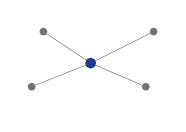
\begin{tikzpicture}[baseline=-2pt]
		\draw[black!45,line width=0.25pt] (0.85,0.45)--(0.10,0.15);
		\draw[black!45,line width=0.25pt] (0.85,0.45)--(0.25,0.85);
		\draw[black!45,line width=0.25pt] (0.85,0.45)--(1.55,0.15);
		\draw[black!45,line width=0.25pt] (0.85,0.45)--(1.65,0.85);
		\fill[Caccnavy] (0.85,0.45) circle (0.07);
		\fill[black!55] (0.10,0.15) circle (0.05);
		\fill[black!55] (0.25,0.85) circle (0.05);
		\fill[black!55] (1.55,0.15) circle (0.05);
		\fill[black!55] (1.65,0.85) circle (0.05);
	\end{tikzpicture}\\[-1pt]
	\textbf{Heterog.\ Graph Builder}\\
	{\tiny $[N{+}1,d_{\text{node}}]$}
	}; \&
	\node[modblock]      (C1) {%
	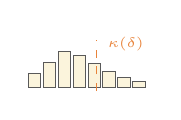
\begin{tikzpicture}[baseline]
		\foreach \x/\h in {0.08/0.18,0.27/0.32,0.46/0.45,0.65/0.4,
				0.84/0.3,1.03/0.2,1.22/0.12,1.41/0.07}{
				\draw[fill=Cbgyellow,draw=black!65,line width=0.3pt]
				(\x,0) rectangle (\x+0.16,\h);}
		\draw[line width=0.6pt,Caccorange,dashed] (0.95,-0.05)--(0.95,0.6);
		\node[font=\tiny,Caccorange] at (1.32,0.55) {$\kappa(\delta)$};
	\end{tikzpicture}\\[-2pt]
	\textbf{Quantile $\kappa(\delta)$}\\
	{\tiny calibration on held-out split}
	}; \&
	\node[modblock]      (D1) {%
	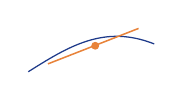
\begin{tikzpicture}[baseline]
		\draw[line width=0.45pt,Caccnavy]
		plot[domain=0:1.6,samples=30,smooth] (\x,{0.1+0.45*sin(\x r * 1.4)});
		\draw[line width=0.55pt,Caccorange] (0.25,0.2)--(1.4,0.65);
		\fill[Caccorange] (0.85,0.43) circle (0.05);
	\end{tikzpicture}\\[-2pt]
	\textbf{SQP Linearization}\\
	{\tiny linearize $g$,\,$h^i_k$ around $\bar{\bm{x}}$}
	}; \&
	\node[modblock]      (E1) {%
	\textbf{eVTOL dynamics}\\[2pt]
	{\small $\bm{x}_{t+1}\!=\!g(\bm{x}_t,\bm{u}_t,\bm{w}_t)$}\\[1pt]
	{\tiny RK4, differentiable}
	}; \\
	% ---- ROW 2 ----
	\node[inputart]      (A2) {%
		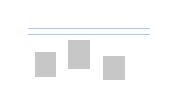
\begin{tikzpicture}[baseline]
			\fill[black!22] (0.08,0.08) rectangle (0.35,0.4);
			\fill[black!22] (0.5,0.18) rectangle (0.78,0.55);
			\fill[black!22] (0.95,0.05) rectangle (1.22,0.35);
			\draw[Cwindblue,line width=0.55pt,opacity=0.75]
			(0,0.62)--(1.55,0.62);
			\draw[Cwindblue,line width=0.55pt,opacity=0.75]
			(0,0.7)--(1.55,0.7);
		\end{tikzpicture}\\[-1pt]
		\textbf{static map}\\
		$\mathcal{M}$: buildings, corridor
	}; \&
	\node[modblock]      (B2) {%
	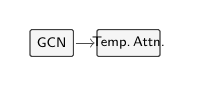
\begin{tikzpicture}[baseline=-2pt]
		\draw[line width=0.4pt,black!75,fill=black!4,rounded corners=0.5pt]
		(0,0) rectangle (0.55,0.34);
		\node[font=\sffamily\tiny] at (0.275,0.17) {GCN};
		\draw[line width=0.4pt,black!75,fill=black!4,rounded corners=0.5pt]
		(0.85,0) rectangle (1.65,0.34);
		\node[font=\sffamily\tiny] at (1.25,0.17) {Temp.\,Attn.};
		\draw[->,line width=0.3pt,black!70] (0.58,0.17)--(0.82,0.17);
	\end{tikzpicture}\\[-1pt]
	\textbf{Spatio-Temp.\ Encoder}\\
	{\tiny $[N{+}1,L,d]\!\to\![N{+}1,d_h]$}
	}; \&
	\node[modblock]      (C2) {%
	\textbf{Nonconformity score}\\[2pt]
	{\scriptsize $s_\theta(\bm{\tau};\bm{\mu},\Sigma)$}\\[-1pt]
	{\tiny $=\min_m(\bm{\tau}{-}\bm{\mu}^m)^{\!\top}\!
		(\Sigma^m)^{-1}(\bm{\tau}{-}\bm{\mu}^m)$}
	}; \&
	\node[novelmod]      (D2) {%
	\textcolor{Caccorange}{$\bigstar$}\,\textbf{Inner Convex QP}\\[2pt]
	{\scriptsize $\min\tfrac12 z^{\!\top}\!Hz+c^{\!\top}\!z$}\\[-1pt]
	{\tiny s.t.\ $Az\!=\!b,\;Gz\!\leq\!h$}\\[-2pt]
	{\tiny \textit{(cvxpylayers backend)}}
	}; \&
	\node[modblock]      (E2) {%
	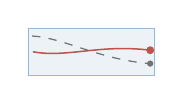
\begin{tikzpicture}[baseline]
		\draw[line width=0.35pt,Cwindblue,fill=Cwindblue,fill opacity=0.18]
		(0,0.1) rectangle (1.6,0.7);
		\draw[line width=0.55pt,Cevtolred]
		(0.06,0.4) .. controls (0.5,0.32) and (0.9,0.5) .. (1.55,0.42);
		\fill[Cevtolred] (1.55,0.42) circle (0.05);
		\draw[line width=0.45pt,black!55,dashed]
		(0.05,0.6) .. controls (0.45,0.58) and (0.9,0.3) .. (1.55,0.25);
		\fill[black!55] (1.55,0.25) circle (0.04);
	\end{tikzpicture}\\[-2pt]
	\textbf{Realized rollout}\\
	{\tiny ego vs.\ neighbor over $T_{\text{end}}$}
	}; \\
	% ---- ROW 3 ----
	\node[inputart]      (A3) {%
		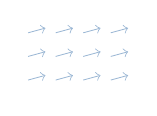
\begin{tikzpicture}[baseline]
			\foreach \x in {0.1,0.45,0.8,1.15}{
					\foreach \y in {0.1,0.4,0.7}{
							\draw[->,line width=0.3pt,Cwindblue]
							(\x,\y)--++(0.22,0.06);}}
		\end{tikzpicture}\\[-1pt]
		\textbf{wind nowcast}\\
		$\hat{\bm{w}}_{t:t+T},\ \Sigma^{w}$
	}; \&
	\node[novelmod]      (B3) {%
	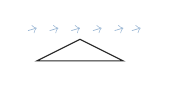
\begin{tikzpicture}[baseline,scale=0.55]
		\draw[line width=0.4pt,black!85] (0.2,0.05)--(1.2,0.55)--(2.2,0.05)--cycle;
		\foreach \x in {0.0,0.5,1.0,1.5,2.0,2.4}{
				\draw[->,line width=0.25pt,Cwindblue]
				(\x,0.75)--++(0.2,0.06);}
	\end{tikzpicture}\\[-2pt]
	\textcolor{Caccorange}{$\bigstar$}\,\textbf{Wind-Cond.\ Cross Attn.}\\
	{\tiny $Q$:\,agents,\ $K{,}V$:\,wind embed}
	}; \&
	\node[modblock]      (C3) {%
	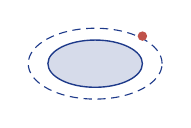
\begin{tikzpicture}[baseline]
		\draw[Caccnavy,line width=0.5pt,fill=Caccnavy,fill opacity=0.18]
		(0.85,0.35) ellipse (0.6 and 0.3);
		\draw[Caccnavy,line width=0.4pt,densely dashed]
		(0.85,0.35) ellipse (0.85 and 0.45);
		\fill[Cevtolred] (1.45,0.7) circle (0.06);
	\end{tikzpicture}\\[-2pt]
	\textbf{Prediction set} $\mathcal{C}^i_{t+k}(\delta)$\\
	{\tiny $\{\bm{\tau}\!:\!s_\theta\!\leq\!\kappa(\delta)\}$}
	}; \&
	\node[modblock]      (D3) {%
	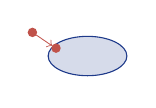
\begin{tikzpicture}[baseline]
		\draw[Caccnavy,line width=0.4pt,fill=Caccnavy,fill opacity=0.18]
		(0.85,0.3) ellipse (0.5 and 0.25);
		\fill[Cevtolred] (0.15,0.6) circle (0.06);
		\fill[Cevtolred] (0.45,0.4) circle (0.06);
		\draw[->,line width=0.3pt,Cevtolred] (0.15,0.6)--(0.4,0.43);
	\end{tikzpicture}\\[-2pt]
	\textbf{CBF separation}\\
	{\tiny $h^i_k\!\geq\!(1{-}\alpha_i)\,h^i_{k-1}$}
	}; \&
	\node[modblock]      (E3) {%
	\textbf{Operational metrics}\\[2pt]
	{\tiny $\Phi_{\text{coll}},\;\Phi_{\text{delay}},$}\\[-1pt]
	{\tiny $\Phi_{\text{lead}},\;\Phi_{\text{energy}}$}
	}; \\
	% ---- ROW 4 ----
	\node[inputart]      (A4) {%
		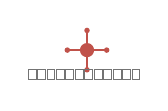
\begin{tikzpicture}[baseline]
			\fill[Cevtolred] (0.8,0.42) circle (0.09);
			\foreach \a in {0,90,180,270}{
					\draw[Cevtolred,line width=0.5pt,
						rotate around={\a:(0.8,0.42)}] (0.8,0.42)--(1.05,0.42);
					\fill[Cevtolred,rotate around={\a:(0.8,0.42)}]
					(1.05,0.42) circle (0.035);}
			\foreach \i in {0,1,...,11}{
					\draw[line width=0.2pt,black!55]
					(0.05+\i*0.12,0.05) rectangle (0.15+\i*0.12,0.18);}
		\end{tikzpicture}\\[-1pt]
		\textbf{ego state}\\
		$\bm{x}_t \!\in\! \mathbb{R}^{12}$
	}; \&
	\node[modblock]      (B4) {%
	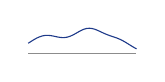
\begin{tikzpicture}[baseline,scale=0.55]
		\draw[line width=0.4pt,Caccnavy]
		plot[domain=0:2.5,samples=40,smooth]
		(\x, {0.4*exp(-3.5*(\x-0.4)^2)
				+ 0.55*exp(-4.0*(\x-1.4)^2)
				+ 0.25*exp(-6.0*(\x-2.1)^2)});
		\draw[line width=0.2pt,black!45] (0,0)--(2.5,0);
	\end{tikzpicture}\\[-2pt]
	\textbf{Multi-Modal GMM Head}\\
	{\tiny $\{\alpha^{i,m}_{t{+}k},\bm{\mu}^{i,m}_{t{+}k},\Sigma^{i,m}_{t{+}k}\}$}
	}; \&
	% --- C4 is the "gradient pass-through" tile, indicating that
	%     back-prop signals also flow through the conformal layer ---
	\node[draw=Caccorange, line width=0.6pt, densely dashed,
	rounded corners=2pt, fill=Cbgyellow, fill opacity=0.5,
	text width=2.95cm, minimum height=1.4cm,
	align=center, font=\sffamily\scriptsize,
	text=Caccorange] (C4) {%
	\textit{gradient}\\
	\textit{pass-through}\\[2pt]
	{\tiny $\partial \mathcal{L}_{\text{TASL}} / \partial \theta$
	\textit{via} $s_\theta$}};
	\&
	\node[novelmod]      (D4) {%
	\textcolor{Caccorange}{$\bigstar$}\,\textbf{Implicit Diff.\ (KKT)}\\[2pt]
	{\scriptsize $\dfrac{\partial \bm{u}^{\star}}{\partial \omega}
		= -M^{-1}\dfrac{\partial F}{\partial \omega}$}
	}; \&
	\node[losshl]        (E4) {%
	\textcolor{Caccorange}{$\bigstar$}\,\textbf{Task-Aligned Loss}\\[2pt]
	{\tiny $\mathcal{L}_{\text{TASL}}\!=\!\lambda_c\widetilde{\Phi}_{\text{coll}}
		\!+\!\lambda_d\Phi_{\text{delay}}$}\\[-1pt]
	{\tiny $\;\;{+}\,\lambda_e\Phi_{\text{energy}}
		\!-\!\lambda_\ell\widetilde{\Phi}_{\text{lead}}
		\!+\!\lambda_a\mathcal{L}_{\text{ADE}}$}
	}; \\
	};

	% ====================================================================
	% Lane backgrounds (drawn behind the matrix via "on background layer")
	% ====================================================================
	\begin{pgfonlayer}{background}
		\node[rounded corners=3pt, fill=Cbggrey, draw=Claneborder,
			line width=0.4pt, inner sep=5pt,
			fit=(A1)(A2)(A3)(A4)] (laneA) {};
		\node[rounded corners=3pt, fill=Cbgblue, draw=Claneborder,
			line width=0.4pt, inner sep=5pt,
			fit=(B1)(B2)(B3)(B4)] (laneB) {};
		\node[rounded corners=3pt, fill=Cbgyellow, draw=Claneborder,
			line width=0.4pt, inner sep=5pt,
			fit=(C1)(C2)(C3)] (laneC) {};
		\node[rounded corners=3pt, fill=Cbggreen, draw=Claneborder,
			line width=0.4pt, inner sep=5pt,
			fit=(D1)(D2)(D3)(D4)] (laneD) {};
		\node[rounded corners=3pt, fill=Cbggrey, draw=Claneborder,
			line width=0.4pt, inner sep=5pt,
			fit=(E1)(E2)(E3)(E4)] (laneE) {};
	\end{pgfonlayer}

	% ====================================================================
	% Lane titles (above each lane background)
	% ====================================================================
	\node[lanetitle, anchor=south, yshift=2pt] at (laneA.north) {(A) Inputs};
	\node[lanesub,  anchor=south, yshift=14pt] at (laneA.north)
	{raw observations};

	\node[lanetitle, anchor=south, yshift=2pt] at (laneB.north)
	{(B) Predictor $f_\theta$};
	\node[lanesub,  anchor=south, yshift=14pt] at (laneB.north)
	{learnable};

	\node[lanetitle, anchor=south, yshift=2pt] at (laneC.north)
	{(C) Conformal};
	\node[lanesub,  anchor=south, yshift=14pt] at (laneC.north)
	{calibration};

	\node[lanetitle, anchor=south, yshift=2pt] at (laneD.north)
	{(D) Safe Planner};
	\node[lanesub,  anchor=south, yshift=14pt] at (laneD.north)
	{differentiable};

	\node[lanetitle, anchor=south, yshift=2pt] at (laneE.north)
	{(E) Closed Loop};
	\node[lanesub,  anchor=south, yshift=14pt] at (laneE.north)
	{\& metrics};

	% ====================================================================
	% Stage banners (above the lane titles, stacked on two rows so they
	% never overlap)
	% Row 1 (closer to titles): Stage 2 -- spans B..E
	% Row 2 (higher up): Stage 1 -- only covers B
	% ====================================================================
	\coordinate (Banner2L) at ([yshift=36pt]laneB.north west);
	\coordinate (Banner2R) at ([yshift=36pt]laneE.north east);
	\node[stagebanner, fill=Cbgyellow, text=Caccorange,
	anchor=south,
	minimum width=14cm]
	at ($(Banner2L)!0.5!(Banner2R)$)
	{Stage 2 (joint fine-tune): $\mathcal{L}_{\text{TASL}}$ via gradient
	loop --- end-to-end across (B)\,\textendash\,(E)};

	\node[stagebanner, fill=Cbgblue, text=Caccnavy,
	minimum width=3.5cm,
	anchor=south] at ([yshift=58pt]laneB.north)
	{Stage 1 (pre-train): $\mathcal{L}_{\text{ADE}}$ only};

	% ====================================================================
	% Forward arrows (inside-lane vertical + inter-lane horizontal)
	% ====================================================================
	% --- Lane A: vertical chain ---
	\draw[fwd] (A1.south) -- (A2.north);
	\draw[fwd] (A2.south) -- (A3.north);
	\draw[fwd] (A3.south) -- (A4.north);

	% --- Lane B: vertical chain ---
	\draw[fwd] (B1.south) -- (B2.north);
	\draw[fwd] (B2.south) -- (B3.north);
	\draw[fwd] (B3.south) -- (B4.north);

	% --- Lane C: vertical chain (3 forward modules + C4 is a gradient
	%     pass-through, connected via a dashed orange arrow upward) ---
	\draw[fwd] (C1.south) -- (C2.north);
	\draw[fwd] (C2.south) -- (C3.north);
	\draw[grad, line width=0.8pt] (C4.north) -- (C3.south);

	% --- Lane D: vertical chain ---
	\draw[fwd] (D1.south) -- (D2.north);
	\draw[fwd] (D2.south) -- (D3.north);
	\draw[fwd] (D3.south) -- (D4.north);

	% --- Lane E: vertical chain ---
	\draw[fwd] (E1.south) -- (E2.north);
	\draw[fwd] (E2.south) -- (E3.north);
	\draw[fwd] (E3.south) -- (E4.north);

	% --- Inter-lane horizontal arrows ---
	% A -> B (4 small arrows from each input artifact)
	\draw[fwd] (A1.east) -- (B1.west);
	\draw[fwd] (A2.east) -- (B2.west);
	\draw[fwd] (A3.east) -- (B3.west);
	\draw[fwd] (A4.east) -- (B4.west);

	% B -> C  (GMM head -> Prediction set)
	% Use an explicit elbow path so the label sits on a horizontal segment.
	\draw[fwd] (B4.east) -- ($(B4.east)+(0.55,0)$)
	|- (C3.west);
	\node[tensorlabel] at ($(B4.east)+(0.55,0.30)$) {$\bm{\mu},\Sigma$};

	% C -> D  (Prediction set -> CBF separation; straight horizontal)
	\draw[fwd] (C3.east) -- (D3.west);
	\node[tensorlabel] at ($(C3.east)!0.5!(D3.west)+(0,0.18)$)
	{$\mathcal{C}^i_{t+k}(\delta)$};

	% D -> E  (Implicit Diff -> eVTOL dynamics)
	% Same elbow trick: label on a horizontal segment.
	\draw[fwd] (D4.east) -- ($(D4.east)+(0.55,0)$)
	|- (E1.west);
	\node[tensorlabel] at ($(D4.east)+(0.55,0.30)$)
	{$\bm{u}_t \!\in\!\mathbb{R}^4$};

	% ====================================================================
	% Gradient feedback arc (smooth bottom sweep, E4 -> D4 -> C -> B4)
	% All routing happens BELOW the lane backgrounds. Annotations sit
	% between the lane bottom and the arc so they never overlap arrows.
	% ====================================================================
	\coordinate (G0) at (E4.south);
	\coordinate (G1) at ($(E4.south) + (0,-1.7)$);
	\coordinate (Gleft) at ($(B4.south) + (0,-1.7)$);
	\coordinate (G5) at ($(B4.south) + (0,-0.4)$);

	% main arc: smooth curve from E4 bottom, sweeping left, into B4 bottom
	\draw[grad]
	(G0) -- (G1)
	.. controls ($(G1) + (-2.5,-0.3)$) and ($(Gleft) + (2.5,-0.3)$) ..
	(Gleft)
	-- (G5) -- (B4.south);

	% Annotations placed between the lane bottoms and the arc.
	% "via KKT" annotation: stacked two lines so it stays narrow and
	%   sits directly under D4 instead of spilling toward the next lane.
	\node[font=\sffamily\tiny\itshape, text=Caccorange,
	anchor=center, align=center,
	fill=white, inner sep=1.5pt]
	at ($(D4.south) + (0,-1.0)$)
	{$\partial \mathcal{L}_{\text{TASL}} / \partial \bm{u}^{\star}$ \\ \textit{via KKT}};

	% (Note: "through s_theta" is already encoded inside C4 itself;
	%  no separate annotation needed.)

	\node[font=\sffamily\tiny\itshape, text=Caccorange,
		anchor=center, align=center,
		fill=white, inner sep=1.5pt]
	at ($(B4.south) + (0,-1.0)$)
	{\textit{updates} $\theta$};

	% ====================================================================
	% Legend (bottom-right)
	% ====================================================================
	\node[draw=Crulegrey, line width=0.4pt, rounded corners=2pt,
		fill=white, inner sep=4pt, anchor=north east,
		font=\sffamily\tiny]
	at ([yshift=-2.6cm]laneE.south east) {%
		\begin{tabular}{@{}l@{\hspace{4pt}}l@{}}
			\tikz \draw[fwd] (0,0)--(0.5,0);
			 & forward data flow          \\[1pt]
			\tikz \draw[grad] (0,0)--(0.5,0);
			 & gradient back-prop         \\[1pt]
			\tikz \fill[Cbgblue,draw=Claneborder,line width=0.2pt]
			(0,0) rectangle (0.3,0.2);
			 & learnable module           \\[1pt]
			\tikz \fill[Cbggreen,draw=Claneborder,line width=0.2pt]
			(0,0) rectangle (0.3,0.2);
			 & diff.\ optimization        \\[1pt]
			\tikz \fill[Cbgyellow,draw=Claneborder,line width=0.2pt]
			(0,0) rectangle (0.3,0.2);
			 & calibration / loss         \\[1pt]
			\textcolor{Caccorange}{$\bigstar$}
			 & contribution of this paper
		\end{tabular}};

\end{tikzpicture}
